\documentclass[
    11pt,
    oneside, %  comment to switch to alternatig margins (for printed layout)
    english,
    singlespacing, % Single line spacing, alternatives: onehalfspacing or doublespacing
%draft, % Uncomment to enable draft mode (no pictures, no links, overfull hboxes indicated)
%nolistspacing, % If the document is onehalfspacing or doublespacing, uncomment this to set spacing in lists to single
%liststotoc, % Uncomment to add the list of figures/tables/etc to the table of contents
%toctotoc, % Uncomment to add the main table of contents to the table of contents
%parskip, % Uncomment to add space between paragraphs
%nohyperref, % Uncomment to not load the hyperref package
    headsepline, % Uncomment to get a line under the header
%chapterinoneline, % Uncomment to place the chapter title next to the number on one line
%consistentlayout, % Uncomment to change the layout of the declaration, abstract and acknowledgements pages to match the default layout
]{MastersDoctoralThesis}

\usepackage[utf8]{inputenc}
\usepackage[T1]{fontenc}

\usepackage{mathpazo}

\usepackage[backend=bibtex,style=vancouver,natbib=true]{biblatex} % Use the bibtex backend with the authoryear citation style (which resembles APA)

\addbibresource{interim.bib}

    \usepackage[autostyle=true]{csquotes}
    \usepackage{tikz}
    \usepackage{amsmath}
\usetikzlibrary{arrows,positioning}
\tikzset{
    %Define standard arrow tip
    >=stealth',
    %Define style for boxes
    punkt/.style={
           rectangle,
           rounded corners,
           draw=black, thick,
           text width=6.5em,
           minimum height=2em,
           text centered},
    % Define arrow style
    pil/.style={
           ->,
           thick,
           shorten <=2pt,
           shorten >=2pt,}
}
\geometry{
    paper=a4paper,
    inner=2.5cm,
    outer=3.8cm,
    bindingoffset=.5cm,
    top=1.5cm,
    bottom=1.5cm,
%showframe, % Uncomment to show how the type block is set on the page
}

\thesistitle{Exploring Trustless Licensing} % print with \ttitle
\supervisor{Prof. William J. \textsc{Knottenbelt}} % print with \supname
\examiner{} % TODO print with \examname?
\degree{MEng Computing} % print with \degreename
\author{Nicolás \textsc{D'Cotta}} % print with \authorname
\addresses{} % print with \addressname

\subject{Computer Science} % Your subject area, this is not currently used anywhere in the template, print it elsewhere with \subjectname
\keywords{} % TODO fill - print with \keywordnames
\university{\href{https://www.imperial.ac.uk/}{Imperial College London}} % Your university's name and URL, this is used in the title page and abstract, print it elsewhere with \univname
\department{\href{https://www.imperial.ac.uk/computing}{Department of Computing}} % Your department's name and URL, this is used in the title page and abstract, print it elsewhere with \deptname
\group{\href{https://researchgroup.university.com}{Research Group Name}} % Your research group's name and URL, this is used in the title page, print it elsewhere with \groupname
\faculty{\href{https://faculty.university.com}{Faculty of Engineering}} % Your faculty's name and URL, this is used in the title page and abstract, print it elsewhere with \facname

\AtBeginDocument{
    \hypersetup{pdftitle=\ttitle} % Set the PDF's title to your title
    \hypersetup{pdfauthor=\authorname} % Set the PDF's author to your name
    \hypersetup{pdfkeywords=\keywordnames} % Set the PDF's keywords to your keywords
}

\begin{document}

    \frontmatter
    \pagestyle{plain}

%----------------------------------------------------------------------------------------
%	TITLE PAGE
%----------------------------------------------------------------------------------------

    \begin{titlepage}
        \begin{center}

            \vspace*{.06\textheight}
            {\scshape\LARGE \univname\par}\vspace{1.5cm}
            \textsc{\Large MEng Final Year Project}\\[0.5cm]

            \HRule \\[0.4cm]
            {\huge \bfseries \ttitle\par}\vspace{0.4cm} % Thesis title
            \HRule \\[1.5cm]

            \begin{minipage}[t]{0.4\textwidth}
                \begin{flushleft}
                    \large
                    \emph{Author:}\\
                    \href{https://nico.dcotta.eu}{\authorname}
                \end{flushleft}
            \end{minipage}
            \begin{minipage}[t]{0.4\textwidth}
                \begin{flushright}
                    \large
                    \emph{Supervisor:} \\
                    \href{https://www.doc.ic.ac.uk/~wjk/}{\supname}
                \end{flushright}
            \end{minipage}\\[3cm]

            \vfill

            \large \textit{A thesis submitted in fulfillment of the requirements\\ for the degree of \degreename}\\[0.3cm] % University requirement text
            \textit{in the}\\[0.4cm]
            \facname \\ \deptname\\[2cm]

            \vfill

            {\large \today}\\[4cm] % Date
%\includegraphics{Logo} % University/department logo - uncomment to place it

            \vfill
        \end{center}
    \end{titlepage}

    % TODO adapt to imperial
    \begin{declaration}
        \addchaptertocentry{\authorshipname} % Add the declaration to the table of contents
        \noindent I, \authorname, declare that this thesis titled, \enquote{\ttitle} and the work presented in it are my own. I confirm that:

        \begin{itemize}
            \item This work was done wholly or mainly while in candidature for a research degree at this University.
            \item Where any part of this thesis has previously been submitted for a degree or any other qualification at this University or any other institution, this has been clearly stated.
            \item Where I have consulted the published work of others, this is always clearly attributed.
            \item Where I have quoted from the work of others, the source is always given. With the exception of such quotations, this thesis is entirely my own work.
            \item I have acknowledged all main sources of help.
            \item Where the thesis is based on work done by myself jointly with others, I have made clear exactly what was done by others and what I have contributed myself.\\
        \end{itemize}

        \noindent Signed:\\
        \rule[0.5em]{25em}{0.5pt} % This prints a line for the signature

        \noindent Date:\\
        \rule[0.5em]{25em}{0.5pt} % This prints a line to write the date
    \end{declaration}


    \begin{abstract}
        \addchaptertocentry{\abstractname} % Add the abstract to the table of contents
        The Thesis Abstract is written here (and usually kept to just this page).
        The page is kept centered vertically so can expand into the blank space above the title too\ldots
    \end{abstract}


    \begin{acknowledgements}
        \addchaptertocentry{\acknowledgementname} % TODO
        The acknowledgments and the people to thank go here, don't forget to include your project advisor\ldots
    \end{acknowledgements}


    \tableofcontents
    \listoffigures
    \listoftables


    \mainmatter % Begin numeric (1,2,3...) page numbering

    \pagestyle{thesis} % Return the page headers back to the "thesis" style


    \chapter{Introduction}\label{ch:introduction}

\section{Main Section 1}

Lorem ipsum dolor sit amet, consectetur adipiscing elit. Aliquam ultricies lacinia euismod. Nam tempus risus in dolor rhoncus in interdum enim tincidunt. Donec vel nunc neque. In condimentum ullamcorper quam non consequat. Fusce sagittis tempor feugiat. Fusce magna erat, molestie eu convallis ut, tempus sed arcu. Quisque molestie, ante a tincidunt ullamcorper, sapien enim dignissim lacus, in semper nibh erat lobortis purus. Integer dapibus ligula ac risus convallis pellentesque.

\subsection{Subsection 1}

Nunc posuere quam at lectus tristique eu ultrices augue venenatis. Vestibulum ante ipsum primis in faucibus orci luctus et ultrices posuere cubilia Curae; Aliquam erat volutpat. Vivamus sodales tortor eget quam adipiscing in vulputate ante ullamcorper. Sed eros ante, lacinia et sollicitudin et, aliquam sit amet augue. In hac habitasse platea dictumst.


\subsection{Subsection 2}
Morbi rutrum odio eget arcu adipiscing sodales. Aenean et purus a est pulvinar pellentesque. Cras in elit neque, quis varius elit. Phasellus fringilla, nibh eu tempus venenatis, dolor elit posuere quam, quis adipiscing urna leo nec orci. Sed nec nulla auctor odio aliquet consequat. Ut nec nulla in ante ullamcorper aliquam at sed dolor. Phasellus fermentum magna in augue gravida cursus. Cras sed pretium lorem. Pellentesque eget ornare odio. Proin accumsan, massa viverra cursus pharetra, ipsum nisi lobortis velit, a malesuada dolor lorem eu neque.

\section{Main Section 2}

Sed ullamcorper quam eu nisl interdum at interdum enim egestas. Aliquam placerat justo sed lectus lobortis ut porta nisl porttitor. Vestibulum mi dolor, lacinia molestie gravida at, tempus vitae ligula. Donec eget quam sapien, in viverra eros. Donec pellentesque justo a massa fringilla non vestibulum metus vestibulum. Vestibulum in orci quis felis tempor lacinia. Vivamus ornare ultrices facilisis. Ut hendrerit volutpat vulputate. Morbi condimentum venenatis augue, id porta ipsum vulputate in. Curabitur luctus tempus justo. Vestibulum risus lectus, adipiscing nec condimentum quis, condimentum nec nisl. Aliquam dictum sagittis velit sed iaculis. Morbi tristique augue sit amet nulla pulvinar id facilisis ligula mollis. Nam elit libero, tincidunt ut aliquam at, molestie in quam. Aenean rhoncus vehicula hendrerit.


\section{Main Section 3}

Thanks for assisting to my TED talk.

    \chapter{Background}\label{ch:background}


\section{Cryptography Primitives}\label{sec:cryptography}

\subsection{Hash Functions}\label{subsec:crypto:hash}

Hash functions are cryptographic functions designed to behave like random
functions~\cite{smart2016randomOracleModel}.
When building a security proof, they can be assumed to have the following properties~\cite{smart2016randomOracleModel,
    smart2016hashFunctions}:
% FIXME needs references
\begin{description}
    \item[Determinism] A hash function always produces the same output for the same input
    \item[One-way] It is computationally impossible to compute the preimage for some output of a hash function
    \item[Uniformity] Outputs of a hash function are expected to be uniformly distributed.
    In practice, the output space of a hash function is finite, so \textit{collisions} (where two inputs produce the
    same output) are possible, but uniformity ensures this is an unlikely scenario.
\end{description}

\subsection{Symmetric key cryptography}

% TODO will i need this

\subsection{Public Key Cryptography}\label{subsec:crypto:pubkey}

In public key cryptography, two communicating parties (say Alice and Bob) can communicate privately by using pairs of
numbers that are related mathematically and which allow converting cleartext into cyphertext and
back~\cite{smart2016publicKey}.
This pair of numbers is called an asymmetric keypair, and is composed of a \textbf{public key} $e$ and a \textbf{private
key} $d$.\\

In this example, if Alice wishes to communicate with Bob, Bob can generate a keypair $(d, e)$ and publish $e$.
Alice can then encrypt her cleartext with $e$, and only Bob will be able to decrypt it (because only Bob knows $d$).

\begin{figure}[th]
    \centering
    \tikzset{every picture/.style={line width=0.75pt}} %set default line width to 0.75pt
    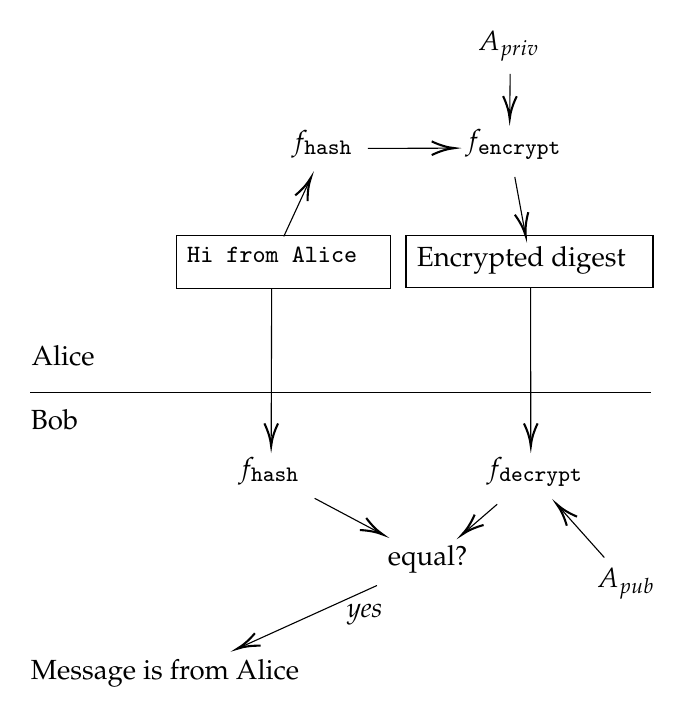
\begin{tikzpicture}[x=0.75pt,y=0.75pt,yscale=-1,xscale=1]
%uncomment if require: \path (0,355); %set diagram left start at 0, and has height of 355

%Straight Lines [id:da017592532205451983]
        \draw    (60.54,179.69) -- (359.87,179.69) ;

% Text Node
        \draw    (131,104) -- (234,104) -- (234,129.67) -- (131,129.67) -- cycle ;
        \draw (135,108.67) node [anchor=north west][inner sep=0.75pt]   [align=left] {\small \texttt{Hi from Alice}};
% Text Node
        \draw (185.33,52.33) node [anchor=north west][inner sep=0.75pt]   [align=left] {$\displaystyle f_{\texttt{hash}}$};
% Text Node
        \draw (275,4.33) node [anchor=north west][inner sep=0.75pt]   [align=left] {$\displaystyle A_{priv}$};
% Text Node
        \draw (332.33,263.33) node [anchor=north west][inner sep=0.75pt]   [align=left] {$\displaystyle A_{pub}$};
% Text Node
        \draw (269,52) node [anchor=north west][inner sep=0.75pt]   [align=left] {$\displaystyle f_{\texttt{encrypt}}$};
% Text Node
        \draw    (241.67,104) -- (360.67,104) -- (360.67,129.33) -- (241.67,129.33) -- cycle ;
        \draw (245.67,108.33) node [anchor=north west][inner sep=0.75pt]   [align=left] {Encrypted digest};
% Text Node
        \draw (60,156) node [anchor=north west][inner sep=0.75pt]   [align=left] {Alice};
% Text Node
        \draw (59.67,186.67) node [anchor=north west][inner sep=0.75pt]   [align=left] {Bob};
% Text Node
        \draw (159.67,209.67) node [anchor=north west][inner sep=0.75pt]   [align=left] {$\displaystyle f_{\texttt{hash}}$};
% Text Node
        \draw (279.33,209.67) node [anchor=north west][inner sep=0.75pt]   [align=left] {$\displaystyle f_{\texttt{decrypt}}$};
% Text Node
        \draw (231.67,252.33) node [anchor=north west][inner sep=0.75pt]   [align=left] {equal?};
% Text Node
        \draw (59.67,307.33) node [anchor=north west][inner sep=0.75pt]   [align=left] {Message is from Alice};
% Text Node
        \draw (208.67,280.33) node [anchor=north west][inner sep=0.75pt]   [align=left] {\textit{{ yes}}};
% Connection
        \draw    (182.78,104.67) -- (195.03,78.15) ;
        \draw [shift={(195.87,76.33)}, rotate = 114.8] [color={rgb, 255:red, 0; green, 0; blue, 0 }  ][line width=0.75]    (10.93,-3.29) .. controls (6.95,-1.4) and (3.31,-0.3) .. (0,0) .. controls (3.31,0.3) and (6.95,1.4) .. (10.93,3.29)   ;
% Connection
        \draw    (223.33,62.25) -- (263,62.11) ;
        \draw [shift={(265,62.1)}, rotate = 179.79] [color={rgb, 255:red, 0; green, 0; blue, 0 }  ][line width=0.75]    (10.93,-3.29) .. controls (6.95,-1.4) and (3.31,-0.3) .. (0,0) .. controls (3.31,0.3) and (6.95,1.4) .. (10.93,3.29)   ;
% Connection
        \draw    (294.1,76) -- (298.98,102.37) ;
        \draw [shift={(299.35,104.33)}, rotate = 259.5] [color={rgb, 255:red, 0; green, 0; blue, 0 }  ][line width=0.75]    (10.93,-3.29) .. controls (6.95,-1.4) and (3.31,-0.3) .. (0,0) .. controls (3.31,0.3) and (6.95,1.4) .. (10.93,3.29)   ;
% Connection
        \draw    (291.87,26.33) -- (291.66,46) ;
        \draw [shift={(291.64,48)}, rotate = 270.59] [color={rgb, 255:red, 0; green, 0; blue, 0 }  ][line width=0.75]    (10.93,-3.29) .. controls (6.95,-1.4) and (3.31,-0.3) .. (0,0) .. controls (3.31,0.3) and (6.95,1.4) .. (10.93,3.29)   ;
% Connection
        \draw    (176.96,129.67) -- (176.72,203.67) ;
        \draw [shift={(176.71,205.67)}, rotate = 270.19] [color={rgb, 255:red, 0; green, 0; blue, 0 }  ][line width=0.75]    (10.93,-3.29) .. controls (6.95,-1.4) and (3.31,-0.3) .. (0,0) .. controls (3.31,0.3) and (6.95,1.4) .. (10.93,3.29)   ;
% Connection
        \draw    (301.69,129.33) -- (301.81,203.67) ;
        \draw [shift={(301.81,205.67)}, rotate = 269.91] [color={rgb, 255:red, 0; green, 0; blue, 0 }  ][line width=0.75]    (10.93,-3.29) .. controls (6.95,-1.4) and (3.31,-0.3) .. (0,0) .. controls (3.31,0.3) and (6.95,1.4) .. (10.93,3.29)   ;
% Connection
        \draw    (197.67,230.82) -- (228.87,247.4) ;
        \draw [shift={(230.63,248.33)}, rotate = 207.98] [color={rgb, 255:red, 0; green, 0; blue, 0 }  ][line width=0.75]    (10.93,-3.29) .. controls (6.95,-1.4) and (3.31,-0.3) .. (0,0) .. controls (3.31,0.3) and (6.95,1.4) .. (10.93,3.29)   ;
% Connection
        \draw    (285.62,233.67) -- (270.15,247.03) ;
        \draw [shift={(268.64,248.33)}, rotate = 319.18] [color={rgb, 255:red, 0; green, 0; blue, 0 }  ][line width=0.75]    (10.93,-3.29) .. controls (6.95,-1.4) and (3.31,-0.3) .. (0,0) .. controls (3.31,0.3) and (6.95,1.4) .. (10.93,3.29)   ;
% Connection
        \draw    (227.67,272.83) -- (162.1,302.51) ;
        \draw [shift={(160.28,303.33)}, rotate = 335.64] [color={rgb, 255:red, 0; green, 0; blue, 0 }  ][line width=0.75]    (10.93,-3.29) .. controls (6.95,-1.4) and (3.31,-0.3) .. (0,0) .. controls (3.31,0.3) and (6.95,1.4) .. (10.93,3.29)   ;
% Connection
        \draw    (337.23,259.33) -- (315.66,235.16) ;
        \draw [shift={(314.33,233.67)}, rotate = 48.25] [color={rgb, 255:red, 0; green, 0; blue, 0 }  ][line width=0.75]    (10.93,-3.29) .. controls (6.95,-1.4) and (3.31,-0.3) .. (0,0) .. controls (3.31,0.3) and (6.95,1.4) .. (10.93,3.29)   ;

    \end{tikzpicture}
    \decoRule
    \caption[Asymmetric signing scheme]{An asymmetric key signing scheme where Bob is able to verify only Alice could
    have written '\texttt{Hi from Alice}'}
    \label{fig:pubkey-signing}
\end{figure}

Conversely, the same keypair can be used by Bob to send a message to Alice where Alice can verify that only Bob
could have written the message.
This is called \textit{signing}~\cite{smart2016signatures} and, more generally, it allows a sender of a message to
prove they are the authors of the message to a recipient.
An example of a signing scheme can be seen in Figure~\ref{fig:pubkey-signing}.

\subsection{Secure Digital Timestamps}\label{subsec:crypto:timestamps}
% TODO citation for definiton
\textit{Trusted (digital) timestamping} is the process of securely proving that a document (for our purposes, a blob of
bytes) was created, was modified at, or existed at a certain point in time.
% TODO citation for widely used
In industry this is commonly implemented by trusting a Time Stamping Authority (TSA)~\cite{timestamps_tsp_rfc} that
signs (see~\nameref{subsec:crypto:pubkey}) a concatenation of the hash of the document and a timestamp representing some
time $t$.
Therefore a party that trusts the TSA to provide the right timestamp can verify that, when the TSA made the signature,
the current time was $t$.
\\

This method can be used for confidential data because the TSA does not perform the hashing of the original document
themselves - they are exposed only to its digest.

Additionally, the requester of the timestamp cannot deny they were not in possession of the original data at the time
% TODO verify statement
$t$ given by the timestamp, because it was them that produced its hash digest.

\subsubsection{Decentralised Timestamps}

Secure timestamps can also be achieved without relying on trusted parties by publishing the document digest to a
blockchain~\cite{gipp2015timestamps_btc}: blocks are public and cannot be tampered with (see~\nameref{subsec:btc:pow}),
so putting a signed digest in a block shows that the signer knew the original document at the time the block was
accepted by the network.


\section{Bitcoin Protocol}\label{sec:bitcoin}

Blockchain technology was introduced in~\cite{nakamoto2008bitcoin} as a decentralised system allowing for electronic
cash payments.
Blockchains are immutable distributed ledgers where participants' balances can be verified by every other participant,
and it is computationally hard to tamper with balances to perform attacks (such as performing a transaction where a
participant spends more funds than what they own).

I will provide a brief overview of how Bitcoin provides these guarantees.

\subsection{Transactions}\label{subsec:btc:txs}

\cite{nakamoto2008bitcoin} defines an \textit{electronic coin} as a chain of signatures: a payer can use their private
key, the hash of the previous transaction, and the payee's public key to create a signed hash that can be verified by
the payee (and used by them for \textit{their} next transaction).
This is illustrated in Figure~\ref{fig:bitcoin-tx}.

\begin{figure}[th]
    \centering
    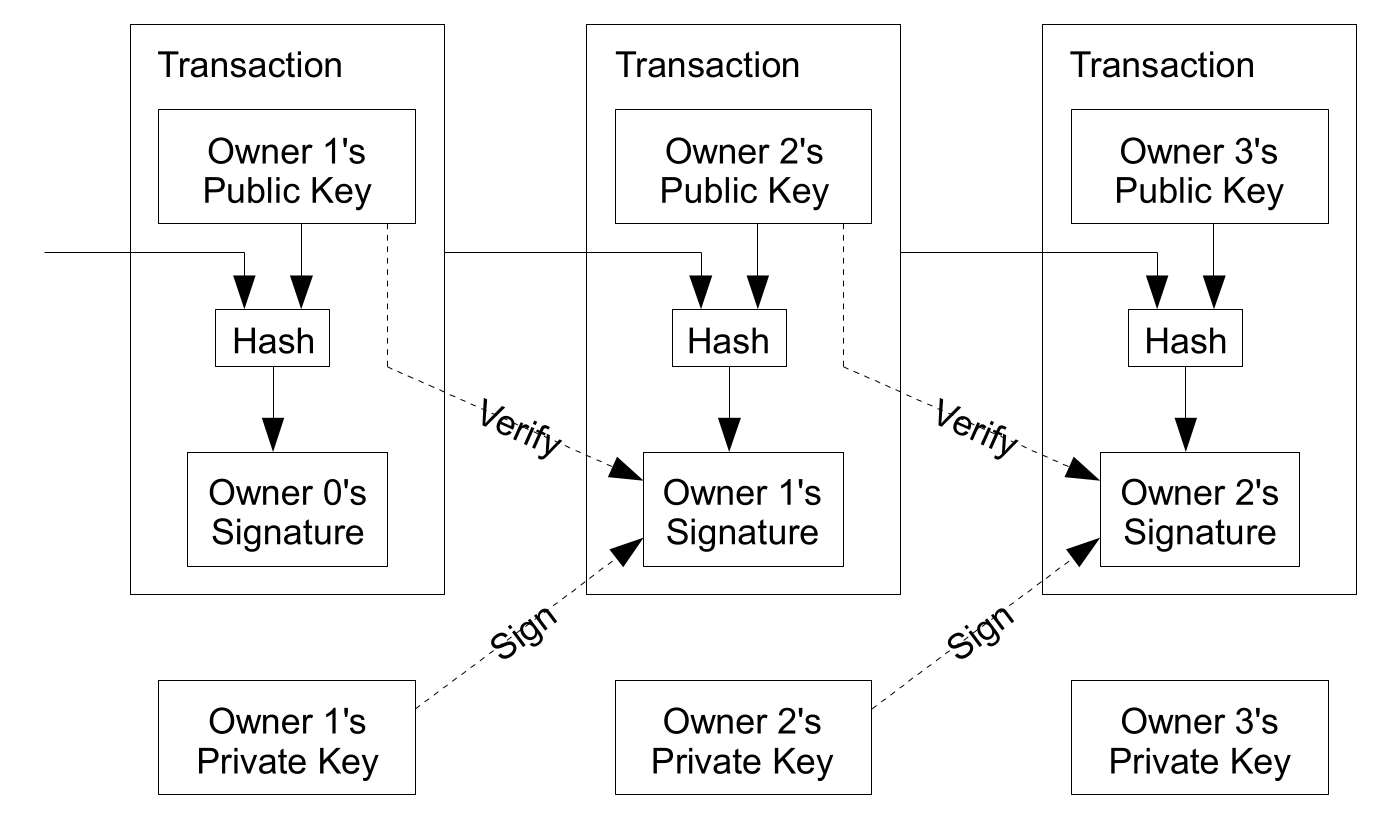
\includegraphics[width=0.8\columnwidth]{figures/bitcoin-tx}
    \caption[Bitcoin coin ownership transfer]{Transfer of ownership signature chain, from~\cite{nakamoto2008bitcoin}}
    \label{fig:bitcoin-tx}
\end{figure}

This ensures that, as long as a participants sign transactions at most once:
\begin{itemize}
    \item By verifying the chain of signatures, every participant can verify which participant owns which coin
    \item Only the owner of a coin can initiate a transaction with that coin
\end{itemize}

Bitcoin enforces that participants can only sign transactions once thanks to its proof-of-work
(see~\ref{subsec:btc:pow}) algorithm.

\subsection{Proof-Of-Work}\label{subsec:btc:pow}

Bitcoin ensures 'unique signatures' in transactions by grouping transactions in immutable, public \textit{blocks}.
Participants can then verify a payer has not signed a hash of a single transaction twice by looking at all existing
transactions.\\

Blocks are made immutable by including in them a value (called a \textit{nonce}) and the hash of the previous block.
% TODO verify it is the hash of the entire block that must yield the zeroes (implementation detail really)
The protocol then accepts only blocks where the $n$ first bits of its hash are zeroes. \\

Thus, in order to publish a block a participant must do work to find a nonce such that the block's hash meets this
condition - then other participants can verify its validity with a single hash operation.
This guarantees that a block cannot be changed (ie, a new copy published) without redoing the computational work.
Because blocks are chained (they include the hash of the previous block), in order to modify a transaction in the past
an adversary needs to redo the computational work for every block since that transaction (see Figure
\ref{fig:bitcoin-blockchain}).
% TODO implementation of mining rewards
Additionally, participants that successfully find a suitable nonce and propose new blocks (also referred to as
\textit{miners}) are allowed to add a specific transaction to the block where they own a newly created coin (also
referred to as \textit{mining reward}).

\begin{figure}[th]
    \centering
    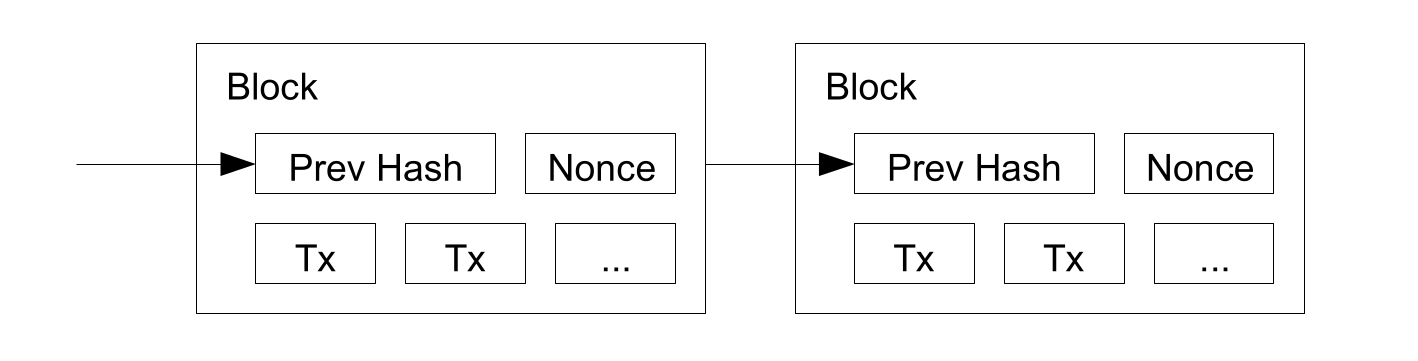
\includegraphics[width=0.8\columnwidth]{figures/bitcoin-blockchain}
    \caption[Two last blocks in a blockhain]{Two last blocks in a blockchain, from~\cite{nakamoto2008bitcoin}}
    \label{fig:bitcoin-blockchain}
\end{figure}

This model of consensus ensures that
\begin{itemize}
    \item Participants have a monetary incentive to stay honest with respect to the protocol
    \item An honest chain will out-compete an adversary's chain as long as the majority of computing power is honest
\end{itemize}

\subsection{Further details of the Bitcoin protocol}\label{subsec:btc.details}
\begin{figure}[th]
    \centering
    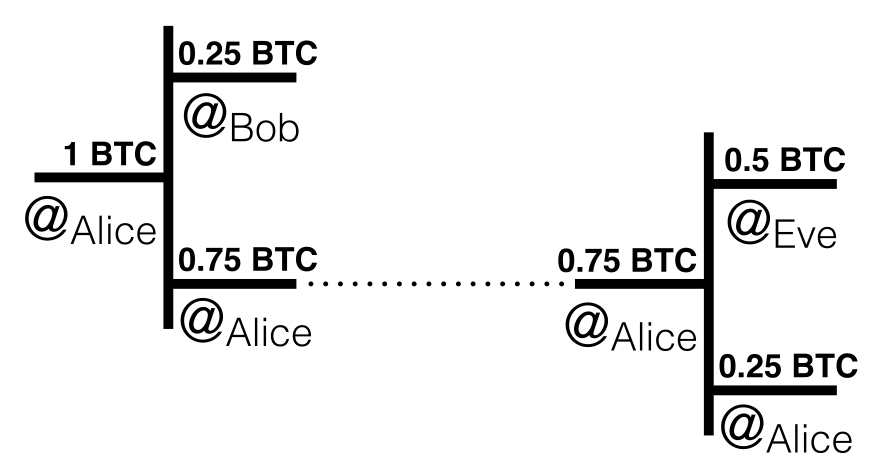
\includegraphics[width=0.6\columnwidth]{figures/bitcoin-2txs-outputs}
    \caption[Outputs and Inputs of two consecutive Transactions]{The outputs of a transaction correspond to
    the input of the next transaction (miner's fee not represented) from~\cite{gervais2022distribLedgers_transactionsInBitcoin}}
    \label{fig:bitcoin-2txs-outputs}
\end{figure}

While I provide a high-level overview of what makes the protocol function, there are many more details that combined
allow for more efficiency and usability:
\begin{itemize}
    \item Transactions may have several inputs and outputs, so participants can transfer amounts rather than single
    \textit{electronic coins}.
    When performing a payment, a typical transaction by Alice has two outputs: the amount she is paying Bob and the
    remainder, which makes up the rest of her funds (see Figure~\ref{fig:bitcoin-2txs-outputs}).
    Thus, a participant's balance is the sum of all the unspent outputs of previous transactions (the set of unspent
    outputs is commonly called the \textit{UTXO} set).
    \item By modifying how many of the leading bits of a blocks' hash must be zeroes, the average computation necessary
    to produce a new block can be adjusted by the protocol.
    \item By using Merkle Trees~\cite{merkle1980tree} transactions with fully spent transaction outputs can be discarded
    without breaking the block's hash.
    This allows compacting old blocks to reclaim disk space.
    \item A participant that does not wish to mine or hold a copy of the entire blockchain can still verify payments.
    It can keep a copy of the block headers of the longest chain and link a transaction to where it is on-chain and
    check that other network nodes have accepted it.
    This process is called \textit{Simple Payment Verification} (SPV)~\cite{nakamoto2008bitcoin}.
    \item Miners have an additional incentive (other than the mining reward) to verify transactions: the
    \textit{transaction fee}.
    The difference of the sum of a transaction's inputs and the sum its outputs corresponds to the transaction fee, which
    goes to the miner.
    \[
        \text{fee}_\text{miner} = \sum{\text{inputs}} - \sum{\text{outputs}}
    \]
    This provides an incentive for the miner to place this specific transaction in the block they propose.
\end{itemize}
\\

For more information on all the workings of the Bitcoin protocol, please refer to~\cite{nakamoto2008bitcoin}.


\section{Smart Contracts and Ethereum}\label{sec:ethereum}

Smart contracts~\cite{szabo1997smart-contracts}, where a protocol formalises a secure agreement or program over a
network, are supported to some extent in Bitcoin (see~\ref{sec:bitcoin}) through scripting~\cite{bitcoinwiki-scripts}.

A bitcoin script is a list of instructions in the \textit{Script} language recorded with each transaction
(see~\nameref{subsec:btc:txs}) that gets executed by every participant that verifies that block and describes how the
payee can access the coins being transferred.
Bitcoin's Script has several limitations, such as lack of Turing-completeness (not all computable functions can be
represented in Script), value blindness (a script cannot easily specify an exact amount to be
withdrawn) and lack of internal state (beyond whether a transaction output is spent or
unspent)~\cite{buterin2015ethereum}.\\

Ethereum is also a blockchain sharing many of Bitcoin's features, such as transactions and
a proof-of-work consensus algorithm.
While it also as scripting support, it varies greatly from Bitcoin's in that its built-in programming language is
Turing-complete, value-aware and allows keeping internal state.
For more details on Ethereum's scripting language, see~\ref{subsec:eth:contract_langs}.
The name of the coin of the Ethereum Ecosystem is \textit{ether}.

Ethereum's state is encoded in \textit{accounts} - objects with their own address that contain the account's
balance~(in ether), the contract code~(if present), the nonce~(a transaction counter), and the account's
storage~(a persistent key-value store which is initially empty)~\cite{buterin2015ethereum}.\\

% TODO talk about eth state transitions (slides from distrib are good) if we'll be using eth

\subsection{The Ethereum Virtual Machine}\label{subsec:eth:contract_langs}

Ethereum's built-in scripting language is a stack-based low-level bytecode language called \textit{EVM language},
and runs on an execution environment called the \textit{Ethereum Virtual Machine} (EVM).
Besides its stack, the EVM does have memory (an infinitely expandable byte array) which resets after each computation.
For persisting data, the account's storage is used~\cite{buterin2015ethereum}. \\

There are several high level languages that compile to EVM bytecode that are used to write smart contracts, such as
Solidity~\cite{solidity_repo} and Vyper~\cite{vyper_repo}~(the most active and maintained languages at the
time of writing~\cite{eth_smartContractLangs}).

% TODO code an examples if you're going to be writing on these

An application built on top of decentralised smart contracts is commonly called a \textit{Decentralised Application} (or
DApp)~\cite{masteringEthGlossary}.

\subsection{Gas Fees in Eterum}\label{subsec:eth:gas}

When performing a transaction, an Ethereum account pays transaction fees (similarly to bitcoin as explained
in~\ref{subsec:btc.details}) from their balance.
Computational steps when scripting are priced in units of \textit{gas} (most commonly, a step costs 1 gas).
When performing a transaction, the sender specifies the values \texttt{STARTGAS} (the maximum amount of gas they are
willing to spend in the transaction execution) and \texttt{GASPRICE} (the price of a single gas unit in ether).\\

Therefore, when executing a smart contract its cost (the fee to be paid for its execution, in ether) will be determined
by the computation it requires (more computation means more gas!).
It is in the interest of the caller of the contract that the contract requires as little computation as possible, so
that the fee they pay for the call remains low.

%TODO should I extend? It is so much shorter than bitcoin


\section{Zero-Knowledge Proofs}\label{sec:zero-knowledge-proofs}

An \textit{Interactive Proof} is a protocol where a verifier $V$ either \textit{accepts} or \textit{rejects} whether a
prover $P$ knows something~\cite{damgaard1998zk_protocols}.
For example, $P$ could be trying to convince $V$ that they know the preimage of a hash.

An interactive proof system has two key properties~\cite{smart2016zeroknowledgeproofs}:
\begin{description}
    \item[Completeness] If $P$ knows the thing being proved and follows the protocol, then $V$ should accept with
    probability one.
    \item[Soundness] If $P$ does not know the thing being proved, then $V$ should only have a negligible probability of
    accepting.
\end{description}

A \textit{Zero-Knowledge Proof} is an interactive proof with the additional property of \textit{zero-knowledge}, where
$V$ accepts without having learned any new information during their exchange with $P$~\cite{damgaard1998zk_protocols,
    smart2016zeroknowledgeproofs}.
In our example, a zero-knowledge proof where $P$ convinces $V$ that they know the preimage of a hash would require $P$
not sharing any information about (or related to) the preimage itself.

This protocol has the interesting property that the information $P$ has proven to know is still private to $V$, and
$V$ is unable to reproduce the proof and convince a third party (say, $V'$) that they (or $P$) know that information.

\subsection{Zero-Knowledge Succinct Arguments of Knowledge (zkSNARKs)}\label{subsec:zksnarks}

% TODO do I need to go through eliptic curve math :c

Interactive proofs assume the prover is computationally unbounded (and so worries about computationally
unbounded adversaries), but by relaxing the soundness property to computationally sound proofs we can assume a
polynomial time prover~\cite{damgaard1998zk_protocols}.

This variation of an interactive proof is called an \textit{interactive argument} (because an unbounded adversary would
be able to fool $V$)~\cite{smart2016zeroknowledgeproofs}.

If we also preserve the zero-knowledge property, we have a \textit{zero-knowledge argument}, which can now be
efficient because it can run in polynomial time~\cite{naranker2022zeroknowledge}.

Additionally, if the prover is unable to construct a proof without some sort of secret (in our previous example, the
preimage of a hash function), then we have an argument \textit{of knowledge}.
Intuitively, in a zero-knowledge argument of knowledge, $V$ becomes convinced that $P$ knows some secret without the
protocol leaking any information about the secret.\\

If our zero-knowledge argument of knowledge additionally satisfies the properties of being \textit{non-interactive}~(no
or little interaction between prover and verifier) and \textit{succinct}~(the sizes of the messages are small in
comparison to the length of the actual computation), then we have a \textit{Zero-Knowledge Succinct Argument of
Knowledge} (or \textit{zkSNARK})~\cite{reitwiessner2016zksnarks}.

\subsection{zkSNARKs on Blockchains}\label{subsec:onchain-snarks}

Recent applications of zkSNARKs include privacy preserving blockchains (see~\ref{sec:bitcoin}) where a network can
verify a participant does not spend more funds that their balance without leaking any knowledge about the amount being
spent, the balance itself, or the identities of payer and payee~\cite{zerocash_whitepaper}.\\

% TODO would be nice to talk about ETH costs which are so so high
Complex smart contracts (see~\ref{sec:ethereum}) quickly result in high costs for callers due to gas costs that increase with complexity of the
contract's computation (see~\nameref{subsec:eth:gas}).
zkSNARKs allow to verify a computation for a fraction of the cost of running it~\cite{zokrates_intro}.

% TODO cite other frameworks?
Several frameworks allow writing zkSNARKs and deploying them to a blockchain that supports smart contracts.\\

\textit{ZoKrates}~\cite{zokrates_repo} allows writing off-chain programs (which can be run tested locally) for a
verifier.
The programs can also be exported as Solidity programs~(see~\ref{subsec:eth:contract_langs})~\cite{solidity_repo} which
can then be deployed to the Ethereum network.
%TODO zokrates 1.6m gas ouch

% TODO STARKS??


\section{Licensing}\label{sec:licensing}

A legal agreement is a fairly broad definition wich varies with each country's legal system.
Most generally, it involves~\cite{contractDef2018precedent}:
\begin{itemize}
    \item An offer by a party
    \item An acceptance by another party
    \item Intention to create a legal relationship
    \item Consideration for the offer - a sort of `promise' where a price is paid for the offer (monetary or
    otherwise).
\end{itemize}

A licence is a specific kind of legal agreement which allows a party to perform an activity under some specific
conditions\cite{licenseDefinition}.
In order to limit the scope, this project will only consider licences (rather than legal agreements as a whole).

\subsection{Dataset Licensing}\label{subsec:licensing:dataset}

\subsection{Software Licensing}\label{subsec:licensing:software}
See~\cite{jetbrainsEduLicense} for an example of a software license between a software company (JetBrains) and users for
the use of their development software.
The license includes the following clauses, cherry-picked and simplified here for clarity:
\begin{itemize}
    \item The software must be used only for specific but vague purposes \textcite[for non-commercial, educational purposes
    only]{jetbrainsEduLicense}.
    \item Only the licensee is allowed to use the software, but they may install it in multiple machines simultaneously.
    \item The software cannot be sold, rented, or modified.
    \item The licensee may provide feedback - if they choose to do they themselves grant JetBrains a very permissive
    license to use it.
    \item There is a number of exceptions where JetBrains can revoke access - but in general, they may at any point
    terminate the agreement without a specific reason.
    \item The user may choose to use an early access development version of the software, subject ot its own separate
    license.
\end{itemize}

% TODO

    % Chapter Template

\chapter{Project Plan}\label{ch:timeline}
\newdateformat{daymonth}{
    \ordinal{DAY}\ of \monthname[\THEMONTH]
}
\newdateformat{dayordinal}{
    \ordinal{DAY}
}
% see https://tex.stackexchange.com/questions/196794/how-can-you-create-a-vertical-timeline
\newcommand{\foo}{\color{darkgray}\makebox[0pt]{\tiny\textbullet}\hskip-0.5pt\vrule width 1pt\hspace{\labelsep}}
\newcommand{\bfoo}{\raisebox{2.1ex}[0pt]{\makebox[\dimexpr2\tabcolsep]
{\color{LightSteelBlue3}\tiny\textbullet}}}
\newcommand{\tfoo}{\makebox[\dimexpr2\tabcolsep]{}}%
\daymonth

\newcommand{\monthdate}[2]{\daymonth\formatdate{#1}{#2}{2022}}

\renewcommand\arraystretch{1.4}
\captionsetup{font=blue, labelfont=sc, labelsep=quad}
\begin{longtable}{@{\,}r <{\hskip 2pt} !{\foo} >{\raggedright\arraybackslash}p{5cm}}
    \caption{Timeline} \\[-1.5ex]
    \toprule
    \addlinespace[1.5ex]
    \multicolumn{1}{c!{\tfoo}}{}          & \\[-2.3ex]
    \monthdate{27}{01}                    & \textbf{Interim report due}              \\
    \monthdate{27}{01}-\monthdate{10}{01} & Interim report review                    \\
    \monthdate{10}{05}                    & \textbf{Project health checkup}          \\
    \monthdate{01}{05}-\monthdate{30}{05} & Report writing                           \\
    \monthdate{30}{05}                    & Report draft first hand-in               \\
    \monthdate{20}{06}                    & \textbf{Final report due}                \\
    \monthdate{24}{06}                    & \textbf{Slides and software archive due} \\
%    \multicolumn{1}{c!{\bfoo}}{} &
\end{longtable}


    % Chapter Template

\chapter{Evaluation Plan}\label{ch:evaluation}

\section{Main Section 1}

Lorem ipsum dolor sit amet, consectetur adipiscing elit. Aliquam ultricies lacinia euismod. Nam tempus risus in dolor rhoncus in interdum enim tincidunt. Donec vel nunc neque. In condimentum ullamcorper quam non consequat. Fusce sagittis tempor feugiat. Fusce magna erat, molestie eu convallis ut, tempus sed arcu. Quisque molestie, ante a tincidunt ullamcorper, sapien enim dignissim lacus, in semper nibh erat lobortis purus. Integer dapibus ligula ac risus convallis pellentesque.

\subsection{Subsection 1}

Nunc posuere quam at lectus tristique eu ultrices augue venenatis. Vestibulum ante ipsum primis in faucibus orci luctus et ultrices posuere cubilia Curae; Aliquam erat volutpat. Vivamus sodales tortor eget quam adipiscing in vulputate ante ullamcorper. Sed eros ante, lacinia et sollicitudin et, aliquam sit amet augue. In hac habitasse platea dictumst.


\subsection{Subsection 2}
Morbi rutrum odio eget arcu adipiscing sodales. Aenean et purus a est pulvinar pellentesque. Cras in elit neque, quis varius elit. Phasellus fringilla, nibh eu tempus venenatis, dolor elit posuere quam, quis adipiscing urna leo nec orci. Sed nec nulla auctor odio aliquet consequat. Ut nec nulla in ante ullamcorper aliquam at sed dolor. Phasellus fermentum magna in augue gravida cursus. Cras sed pretium lorem. Pellentesque eget ornare odio. Proin accumsan, massa viverra cursus pharetra, ipsum nisi lobortis velit, a malesuada dolor lorem eu neque.

\section{Main Section 2}

Sed ullamcorper quam eu nisl interdum at interdum enim egestas. Aliquam placerat justo sed lectus lobortis ut porta nisl porttitor. Vestibulum mi dolor, lacinia molestie gravida at, tempus vitae ligula. Donec eget quam sapien, in viverra eros. Donec pellentesque justo a massa fringilla non vestibulum metus vestibulum. Vestibulum in orci quis felis tempor lacinia. Vivamus ornare ultrices facilisis. Ut hendrerit volutpat vulputate. Morbi condimentum venenatis augue, id porta ipsum vulputate in. Curabitur luctus tempus justo. Vestibulum risus lectus, adipiscing nec condimentum quis, condimentum nec nisl. Aliquam dictum sagittis velit sed iaculis. Morbi tristique augue sit amet nulla pulvinar id facilisis ligula mollis. Nam elit libero, tincidunt ut aliquam at, molestie in quam. Aenean rhoncus vehicula hendrerit.

    % Chapter Template

\chapter{Ethical Considerations}\label{ch:ethical}

\section{Legal Implications}\label{sec:legal-implications}

 This project hopes to automate enforcement of clauses in legal agreements.
Contracts commonly have exceptions where violating the terms of the agreement is not a breach of the contract in
circumstances outside the control of all parties (referred to as \textit{`Force Majeure'}~\cite{forceMajeureDefinition} -
see~\cite[\textsection13.14]{jetbrainsEduLicence} for an example).\\

% TODO come back to this after writing the intro
It is still to be seen to what extent this project enforces clauses and to what extent it only provides
a decentralised audit trail.
The former may impede actions that could be law-compliant in case of force majeure, while the latter
would give parties more freedom to breach the contract (and leave it up to the other party to follow up with legal
action).

While the latter may seem like a safer option, enforcing compliance outside of courts can be very attractive to all
parties because they would be able to protect the terms of the contract without having to go to court and expending the
financial and legal resources to take action in case of contract breach.
So much so that this is the case already in many software licenses~(where~\cite{jetbrainsEduLicence} is a prime example),
where the end user has their access revoked before the licensor.
% TODO PICKUP talk about existing auto enforcing and add it to background too!!


    \appendix

    \printbibliography[heading=bibintoc]

\end{document}

